\chapter{Matrizes de Confusão}
\label{ap:matrizes_de_confusao}

\begin{figure}[!ht]
    \centering
	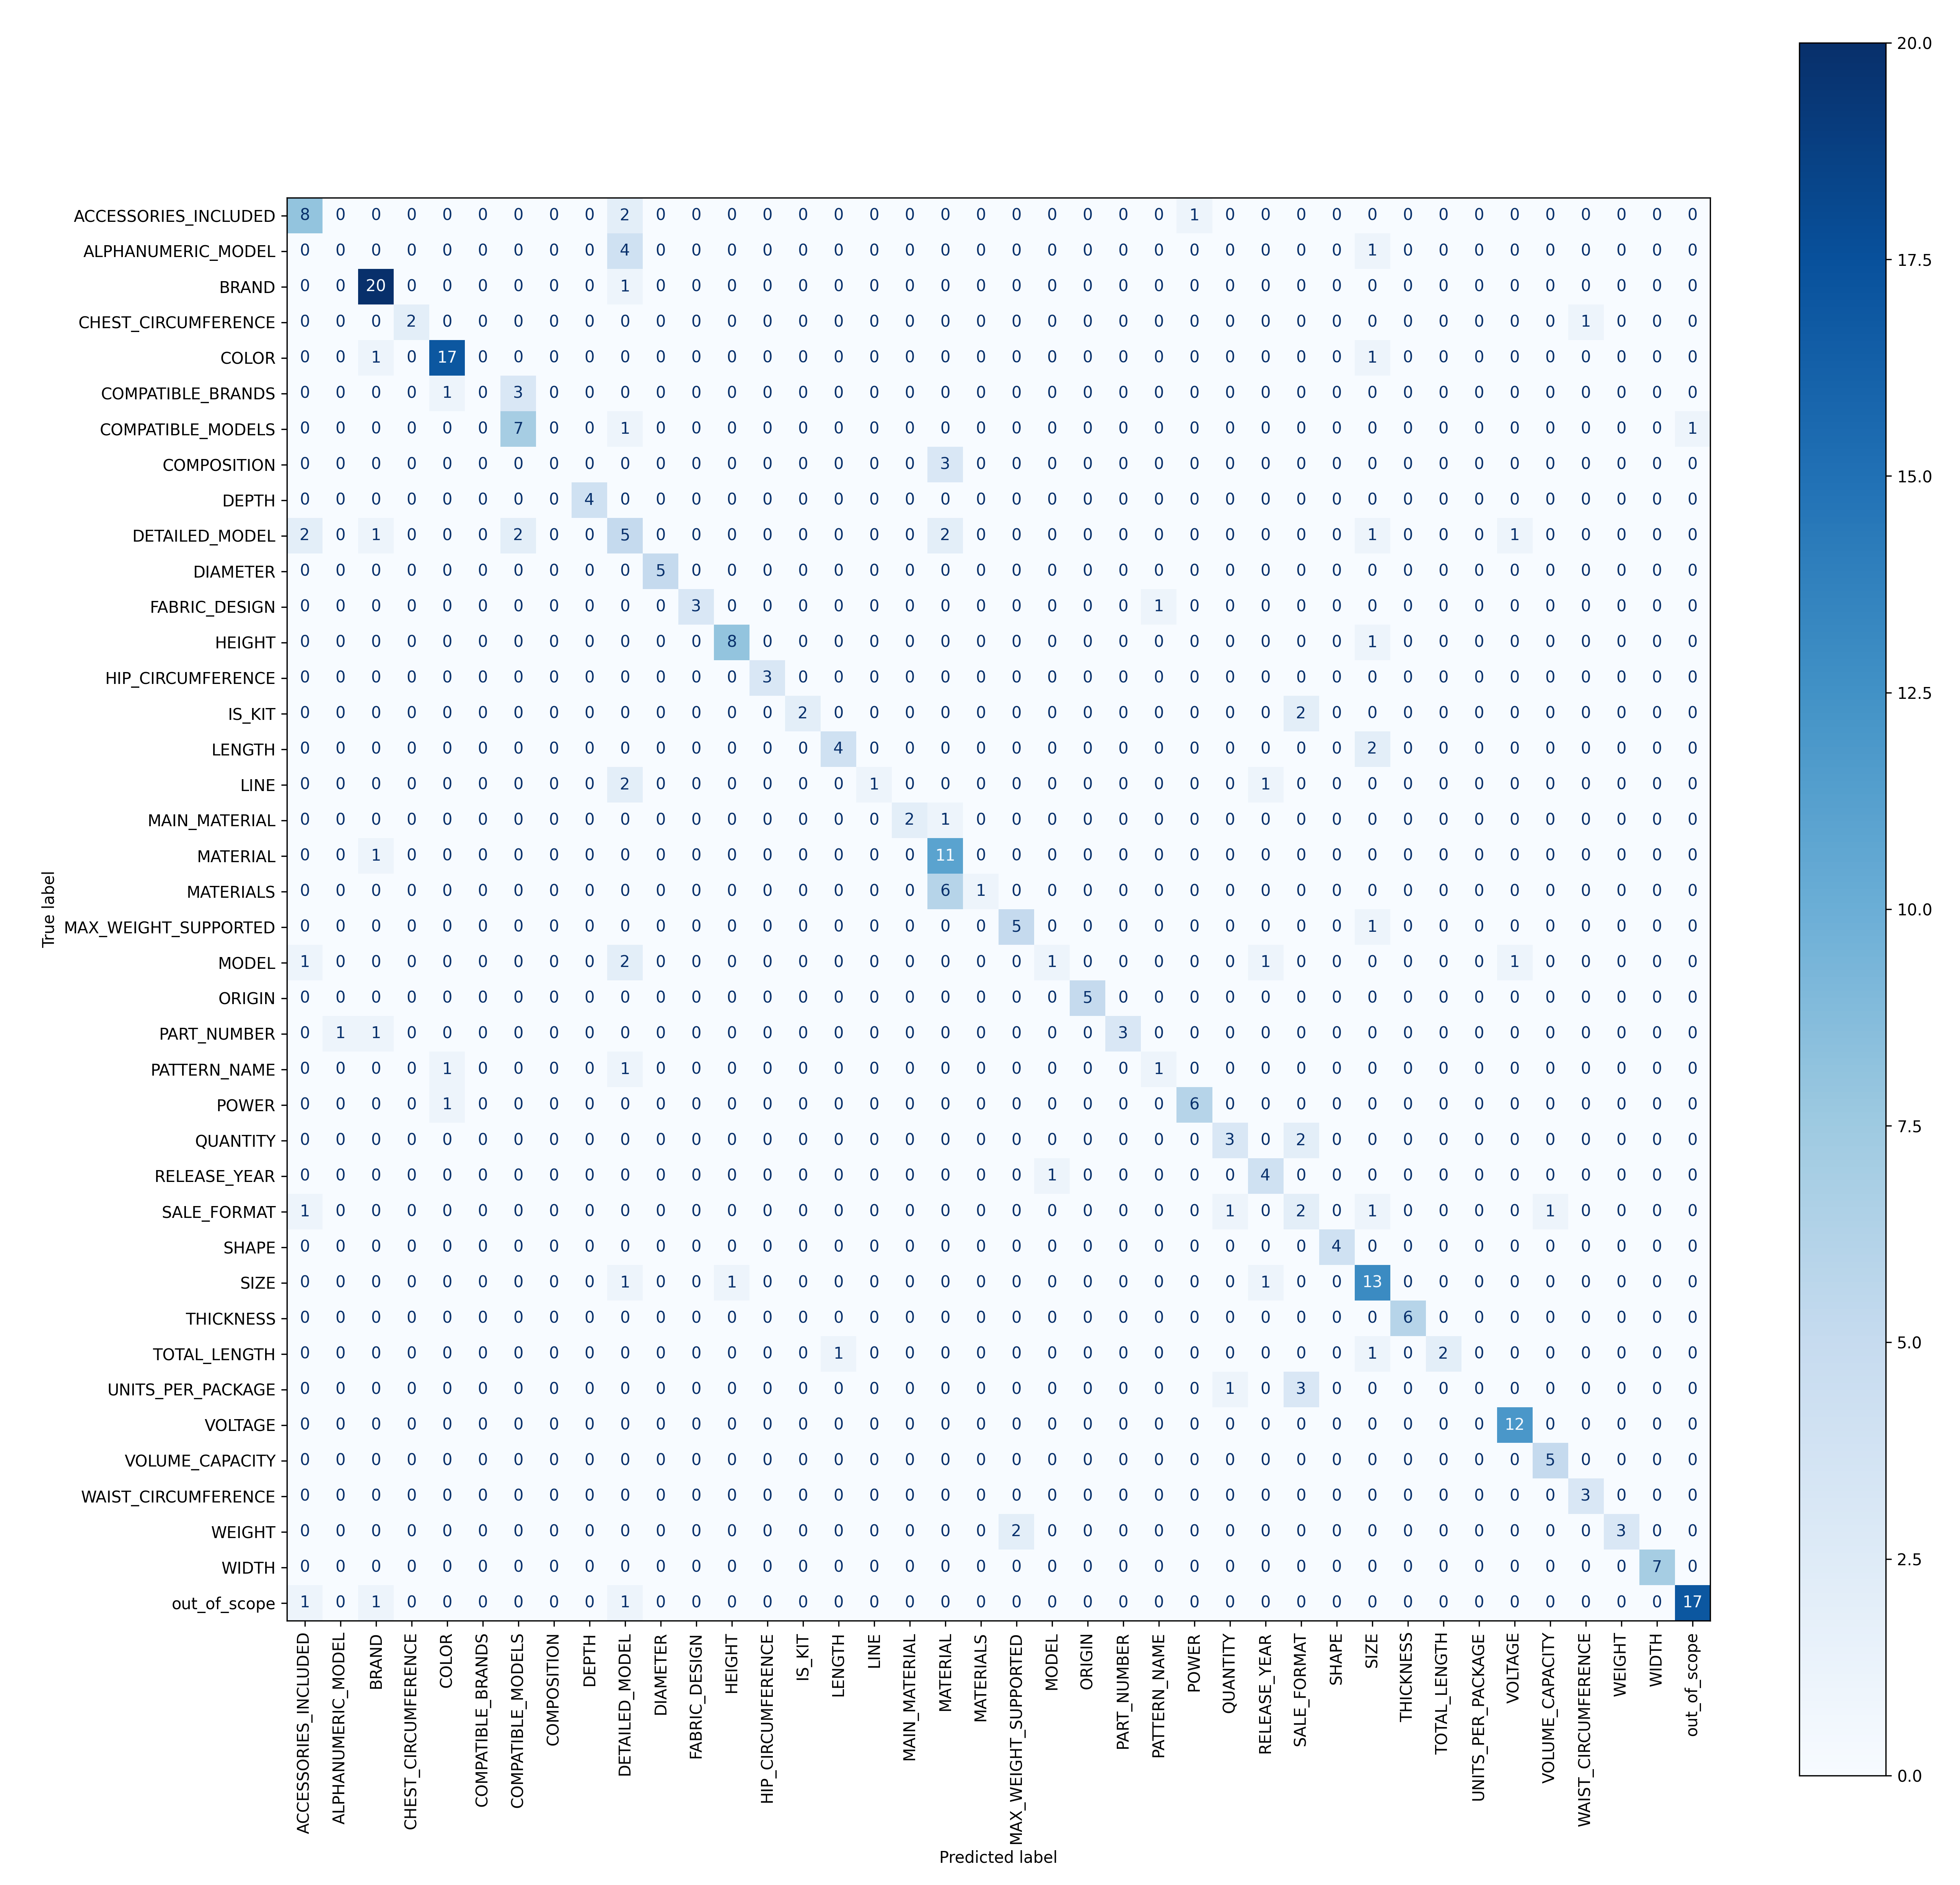
\includegraphics[width=1\linewidth]{figuras/HF1.png}
	\caption{Matriz de Confusão gerada após teste do modelo HF1, na configuração com 40 classes.}
	\label{fig:matriz_hf1}
\end{figure}

\begin{figure}[!ht]
    \centering
	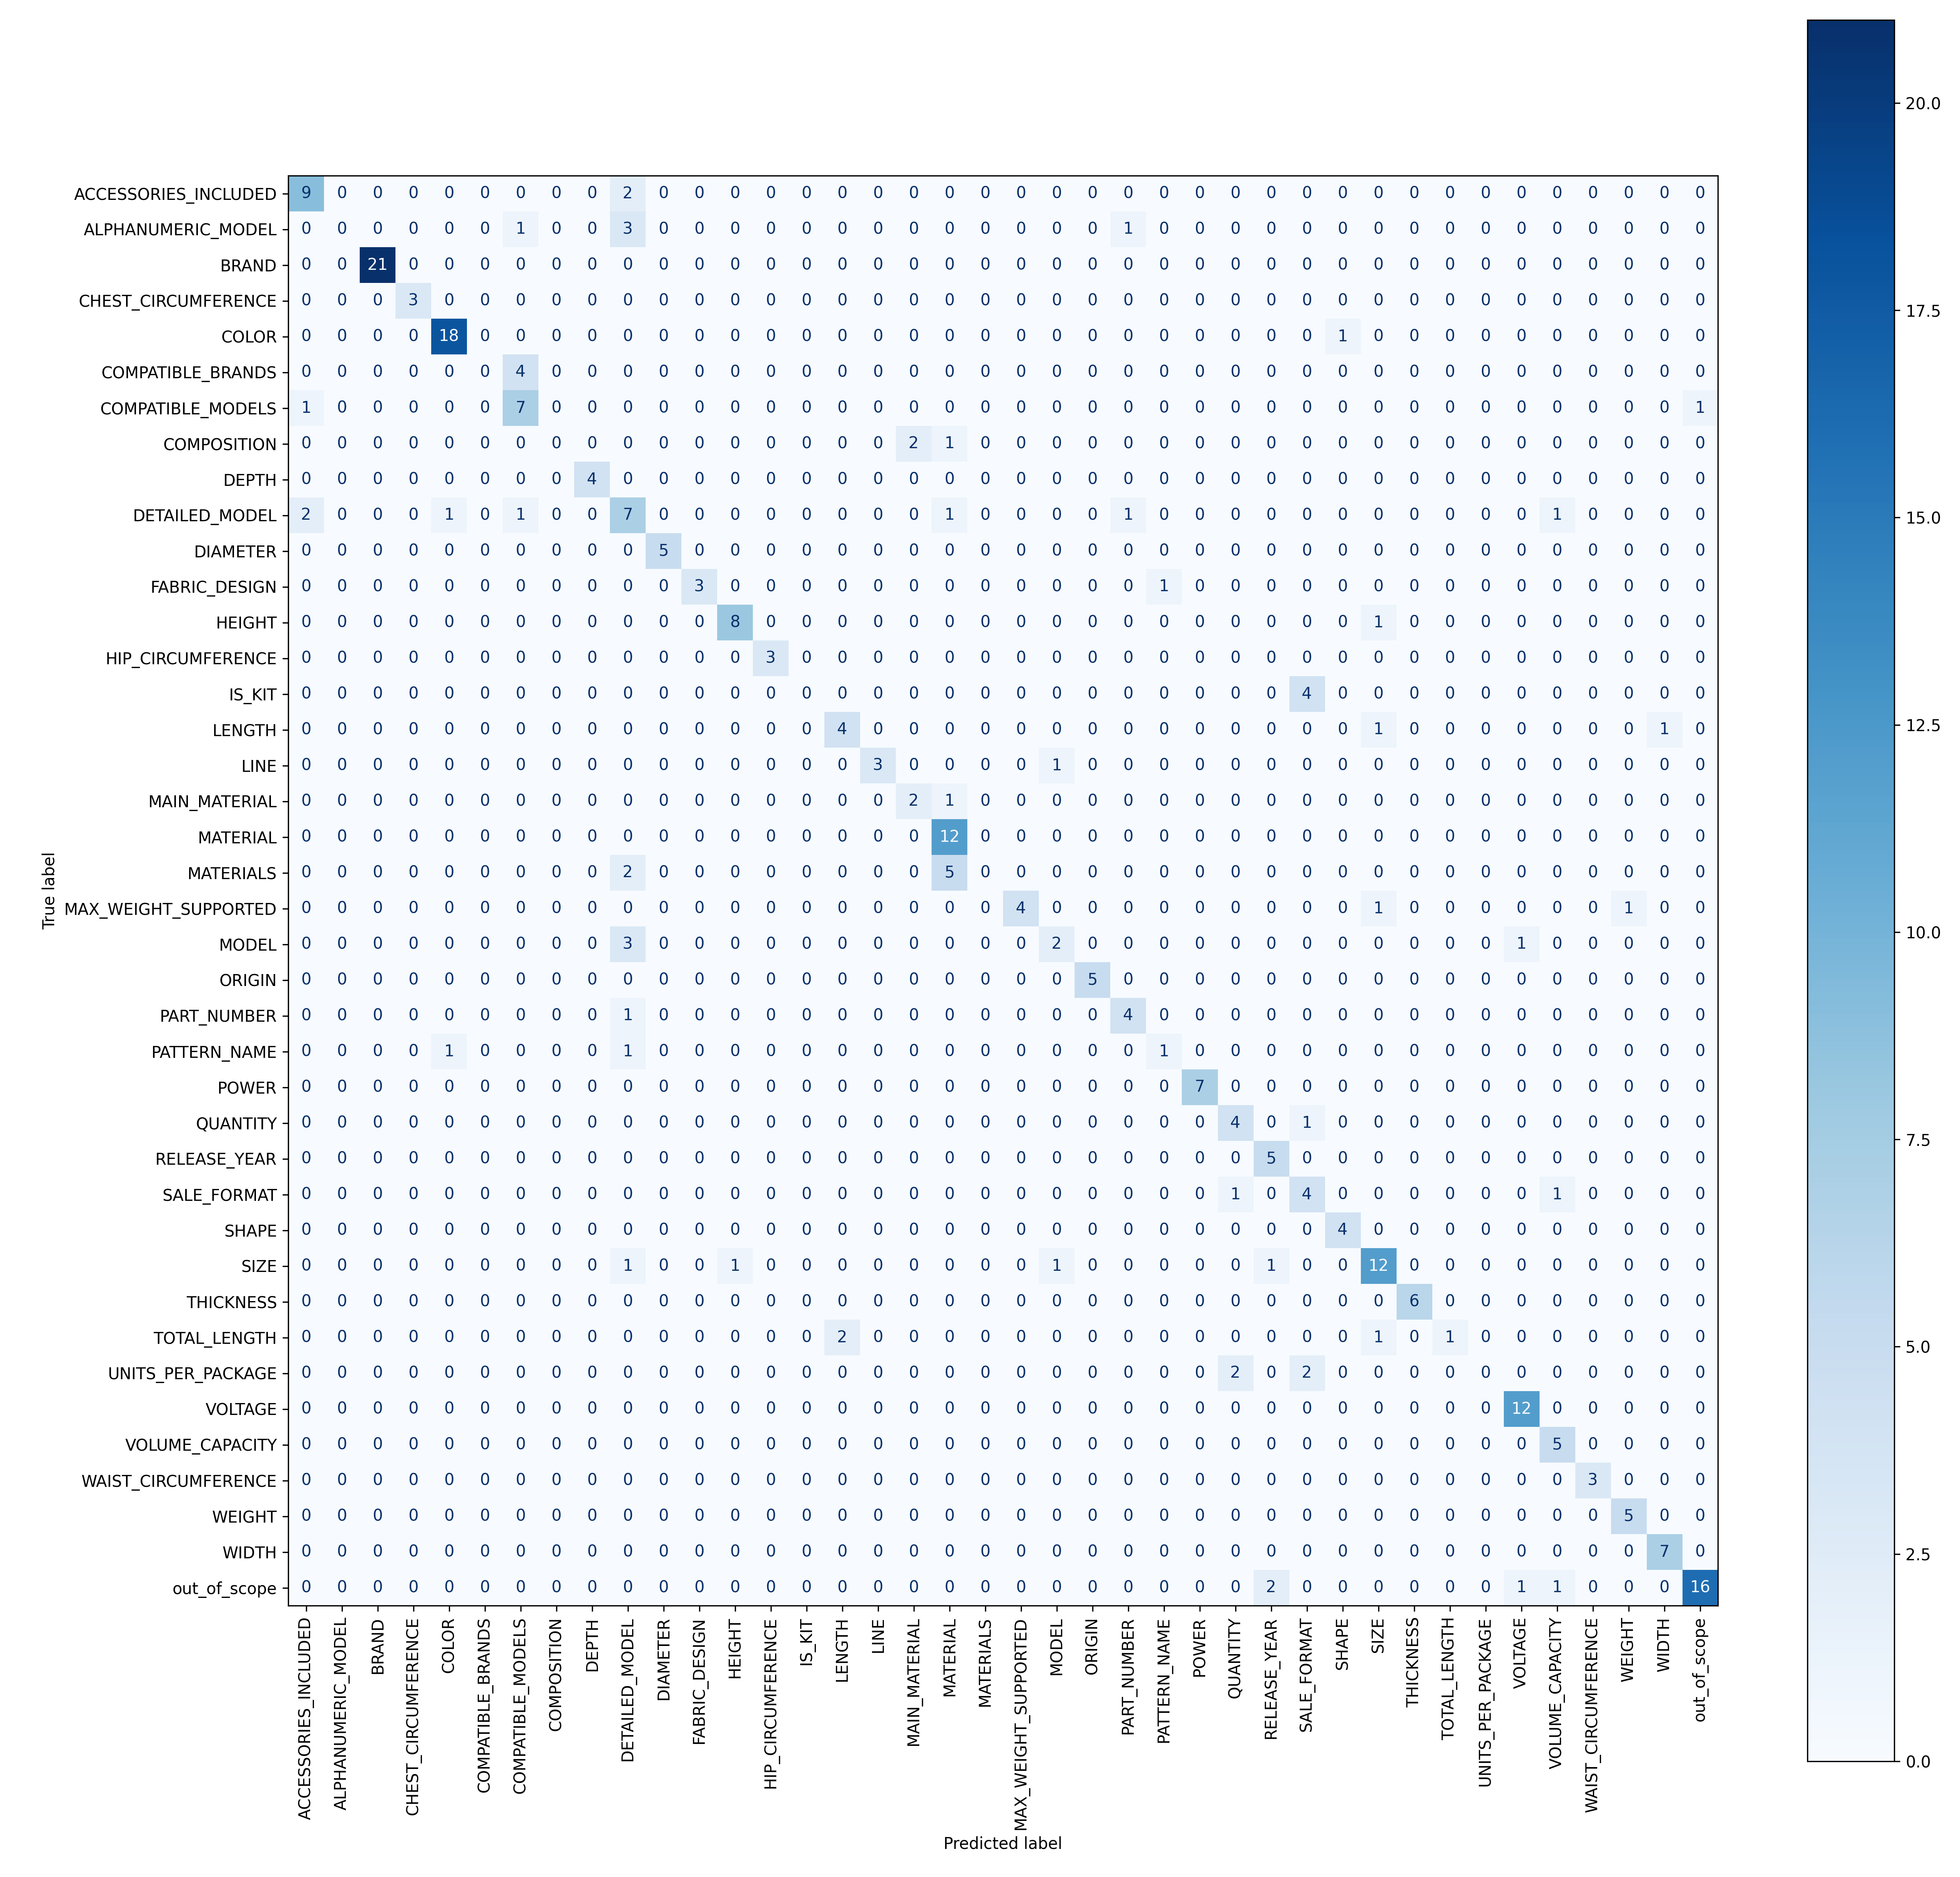
\includegraphics[width=1\linewidth]{figuras/HF2.png}
	\caption{Matriz de Confusão gerada após teste do modelo HF2, na configuração com 40 classes.}
	\label{fig:matriz_hf2}
\end{figure}

\begin{figure}[!ht]
    \centering
	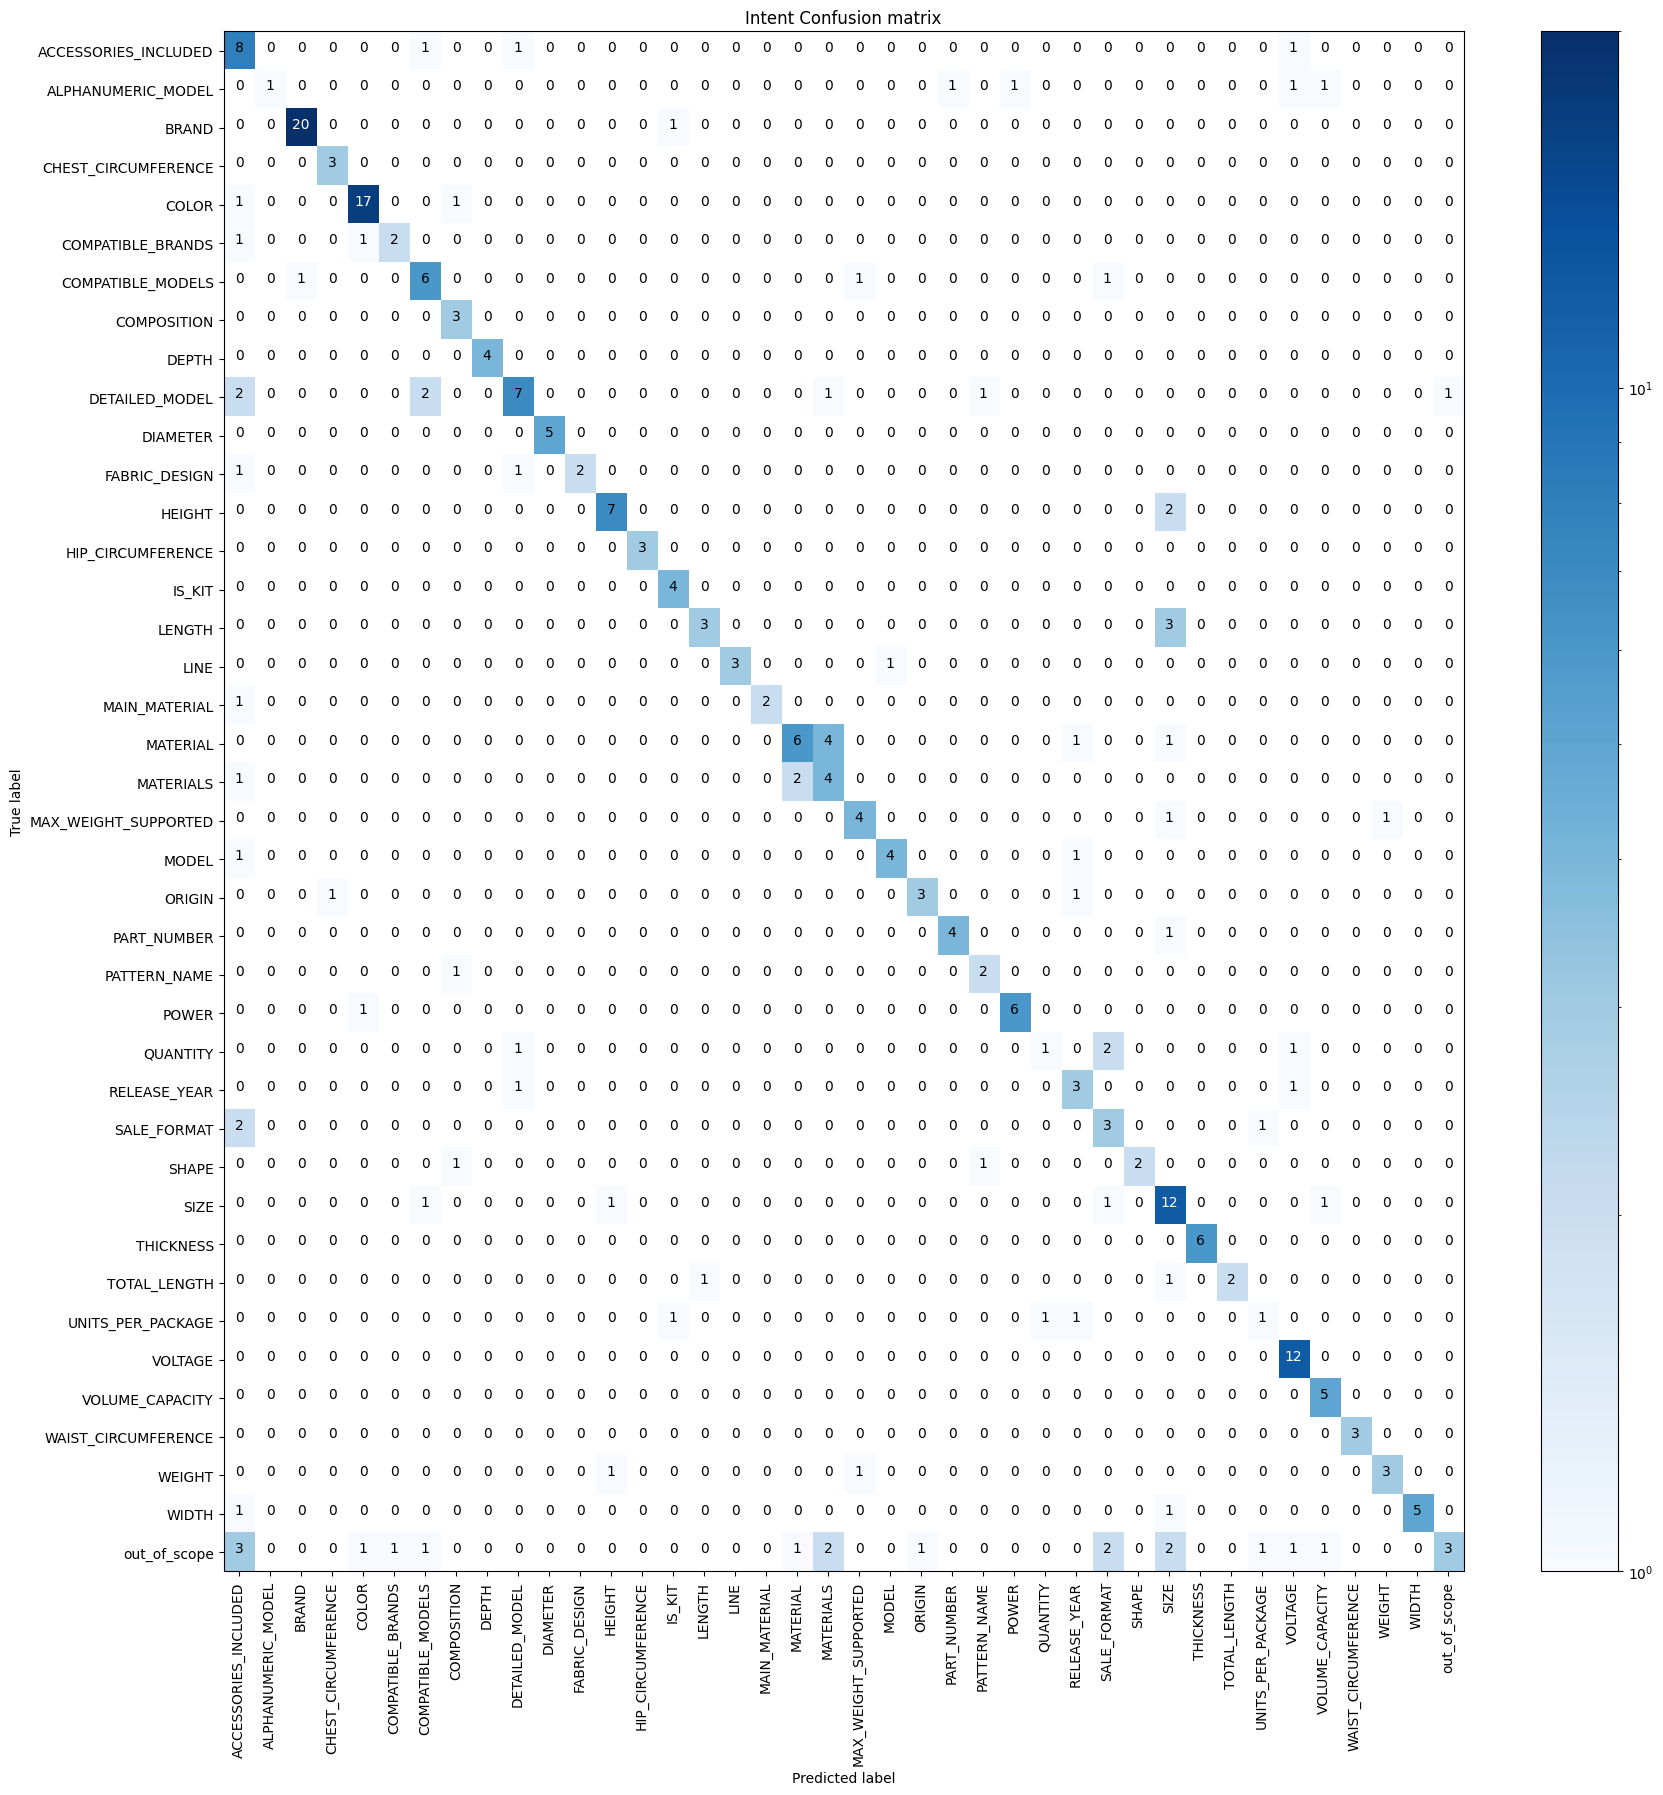
\includegraphics[width=1\linewidth]{figuras/RASA1.png}
	\caption{Matriz de Confusão gerada após teste do modelo RASA1, na configuração com 40 classes.}
	\label{fig:matriz_rasa1}
\end{figure}

\begin{figure}[!ht]
    \centering
	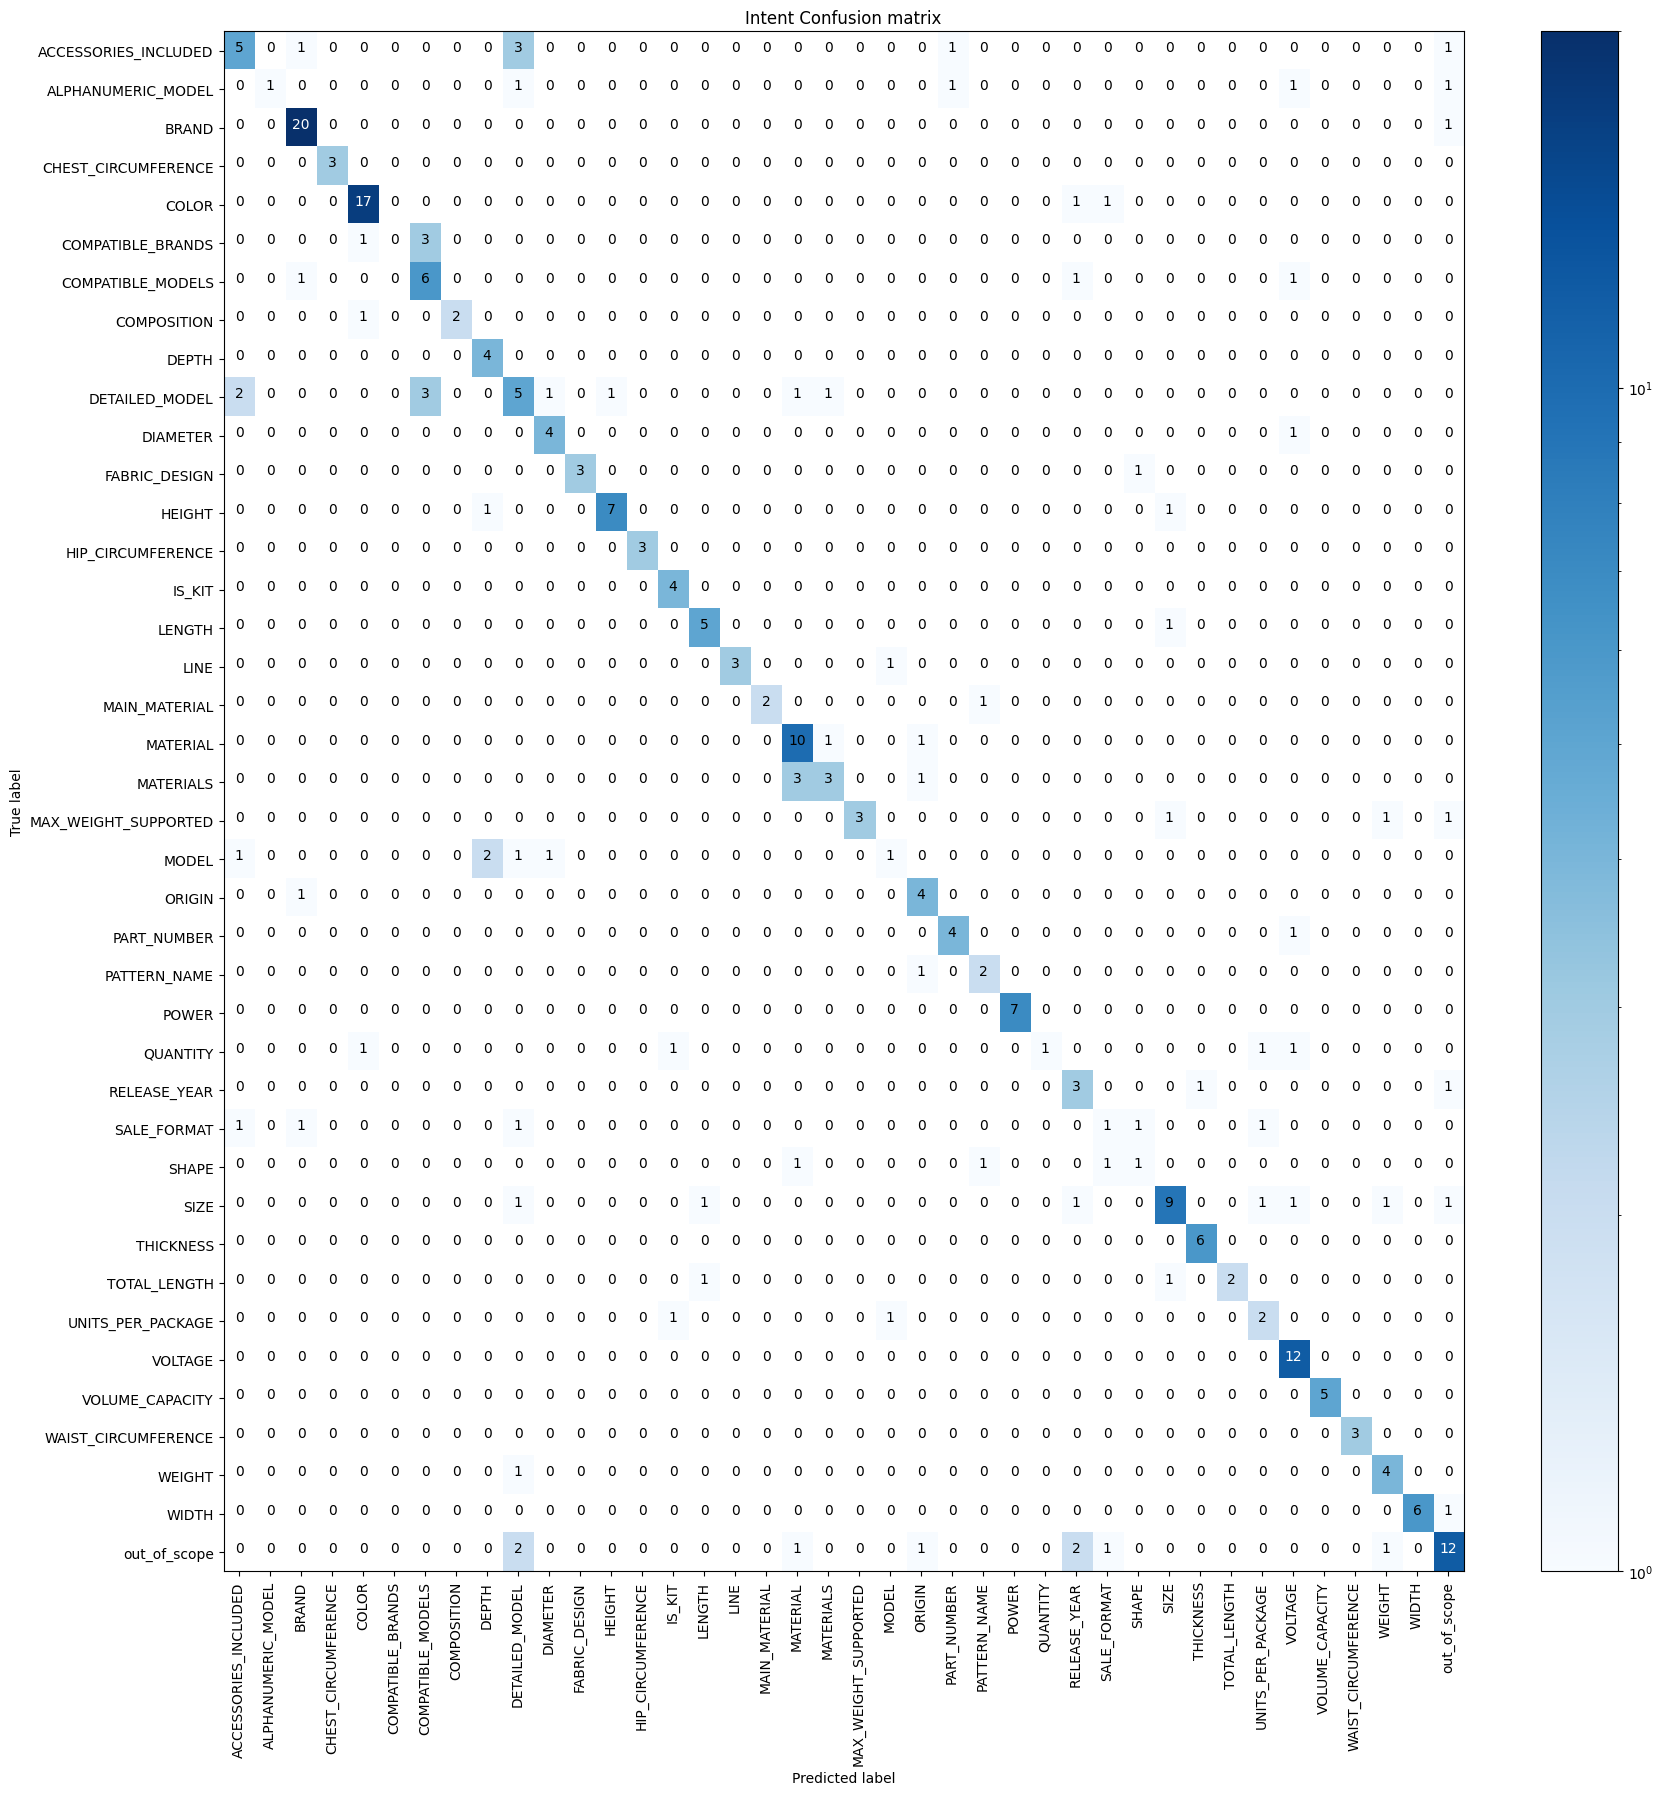
\includegraphics[width=1\linewidth]{figuras/RASA2.png}
	\caption{Matriz de Confusão gerada após teste do modelo RASA2, na configuração com 40 classes.}
	\label{fig:matriz_rasa2}
\end{figure}

\begin{figure}[!ht]
    \centering
	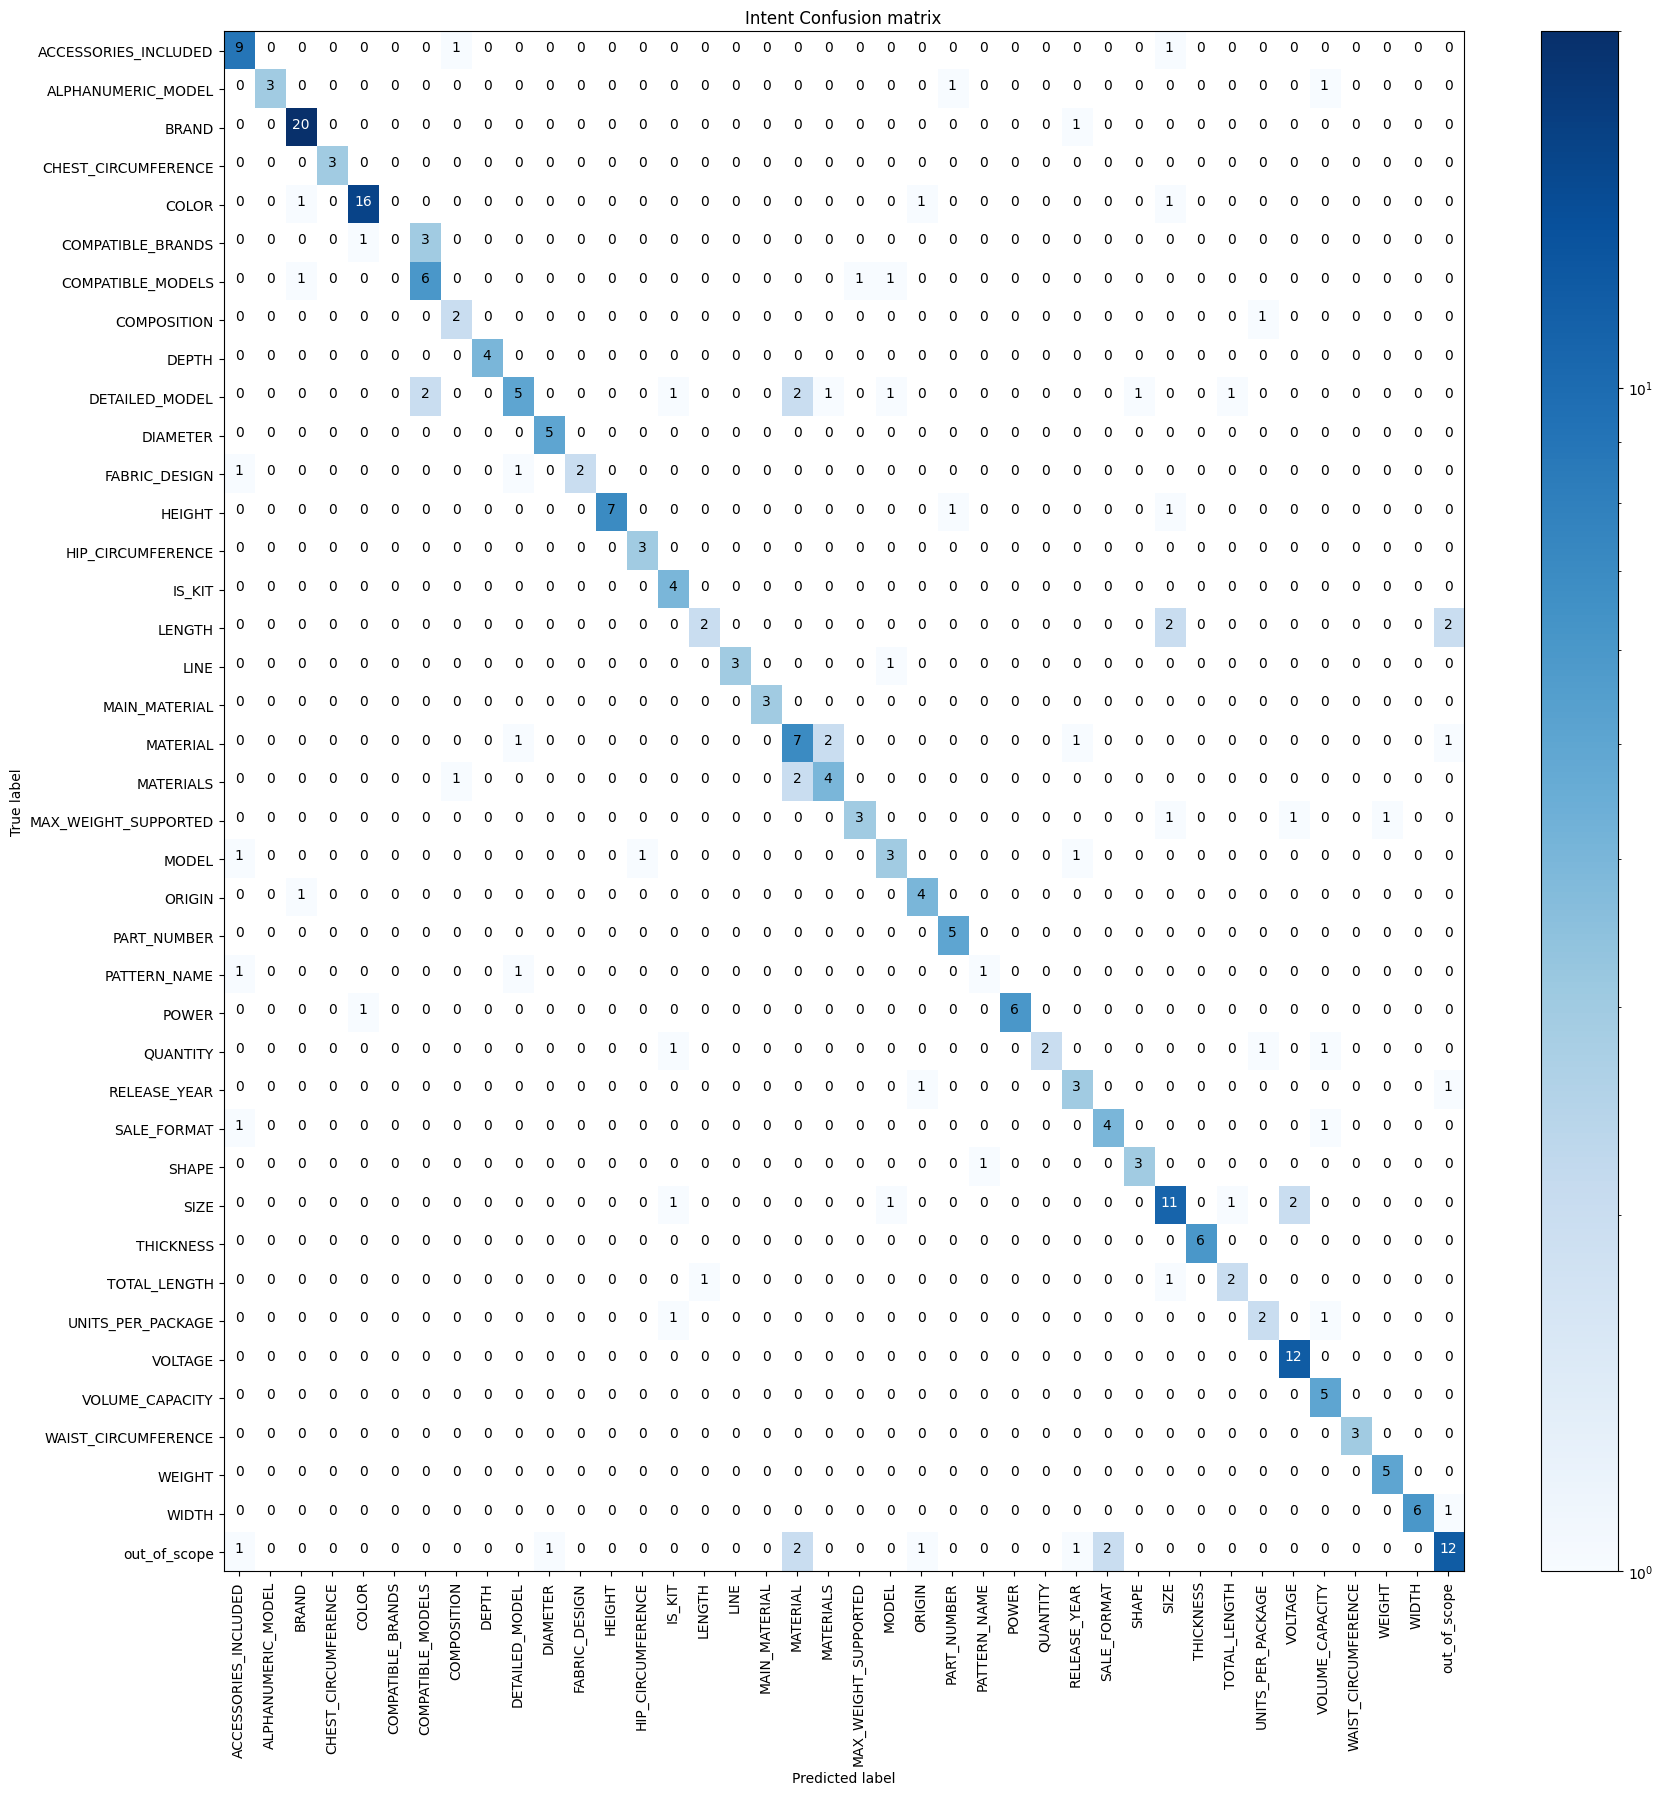
\includegraphics[width=1\linewidth]{figuras/RASA3.png}
	\caption{Matriz de Confusão gerada após teste do modelo RASA3, na configuração com 40 classes.}
	\label{fig:matriz_rasa3}
\end{figure}

\begin{figure}[!ht]
    \centering
	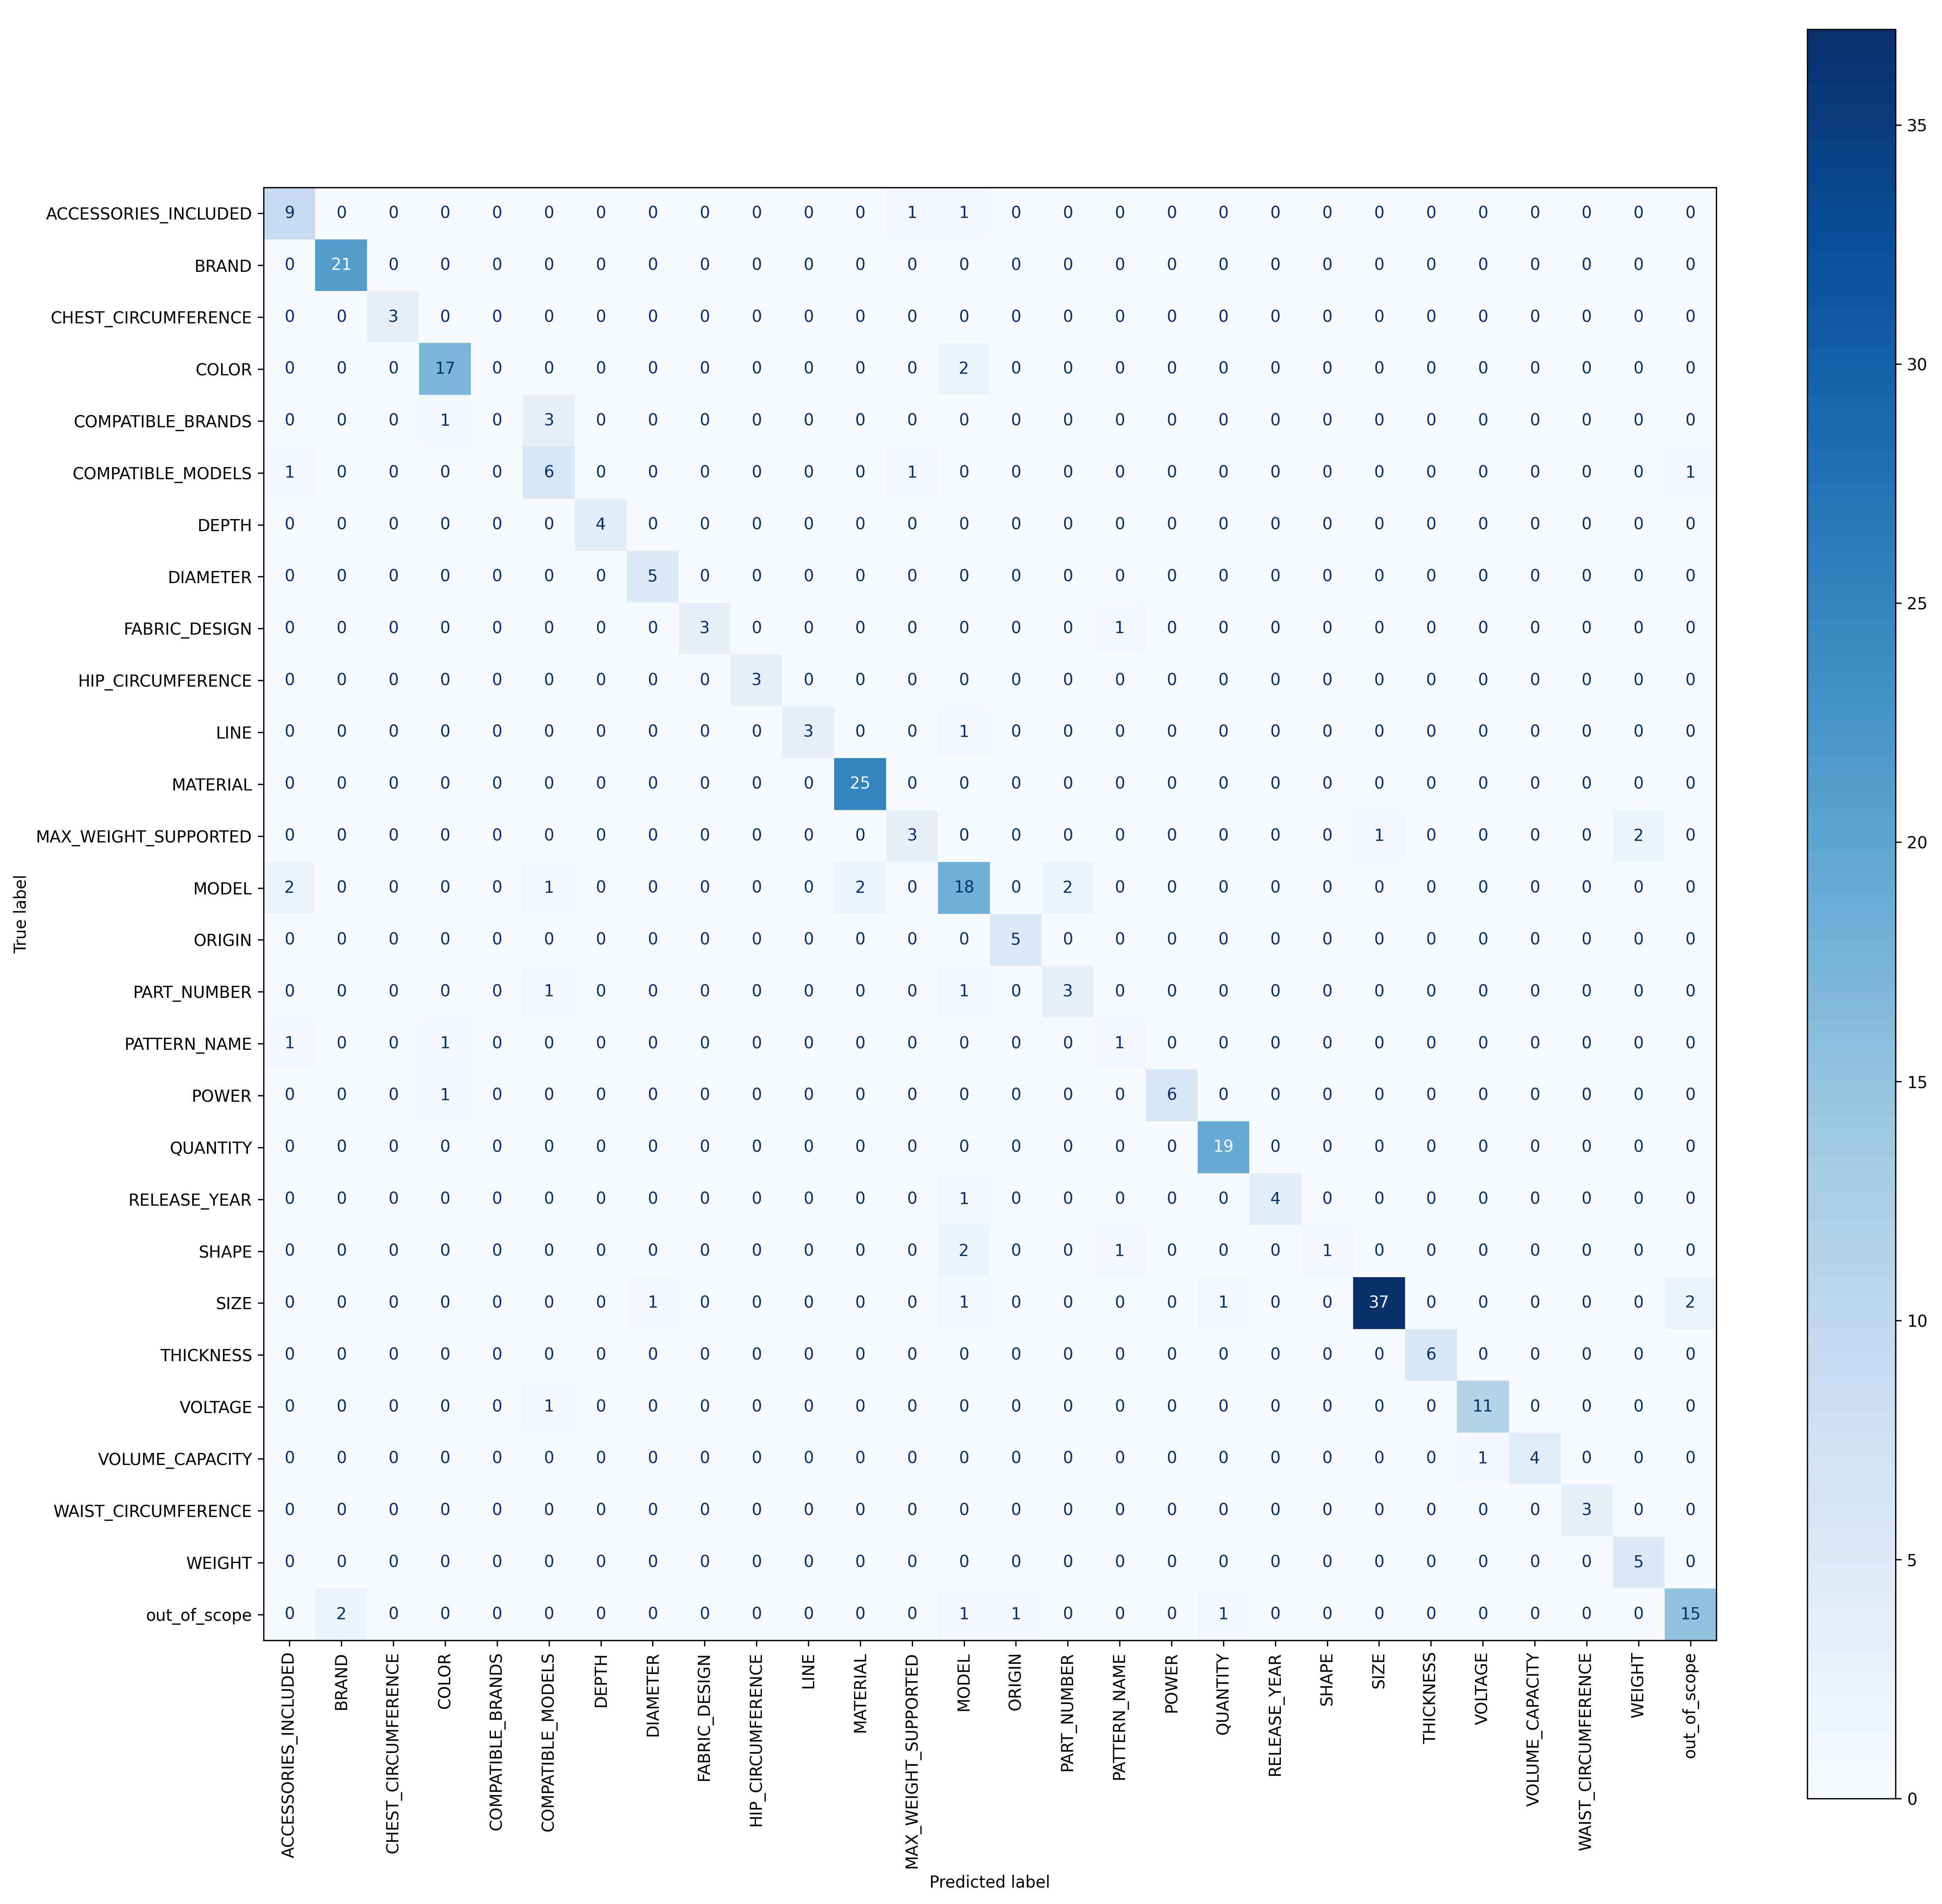
\includegraphics[width=1\linewidth]{figuras/HF2-28_classes.png}
	\caption{Matriz de Confusão gerada após teste do modelo HF2, na configuração com 28 classes.}
	\label{fig:matriz_hf2_28_classes}
\end{figure}

\begin{figure}[!ht]
    \centering
	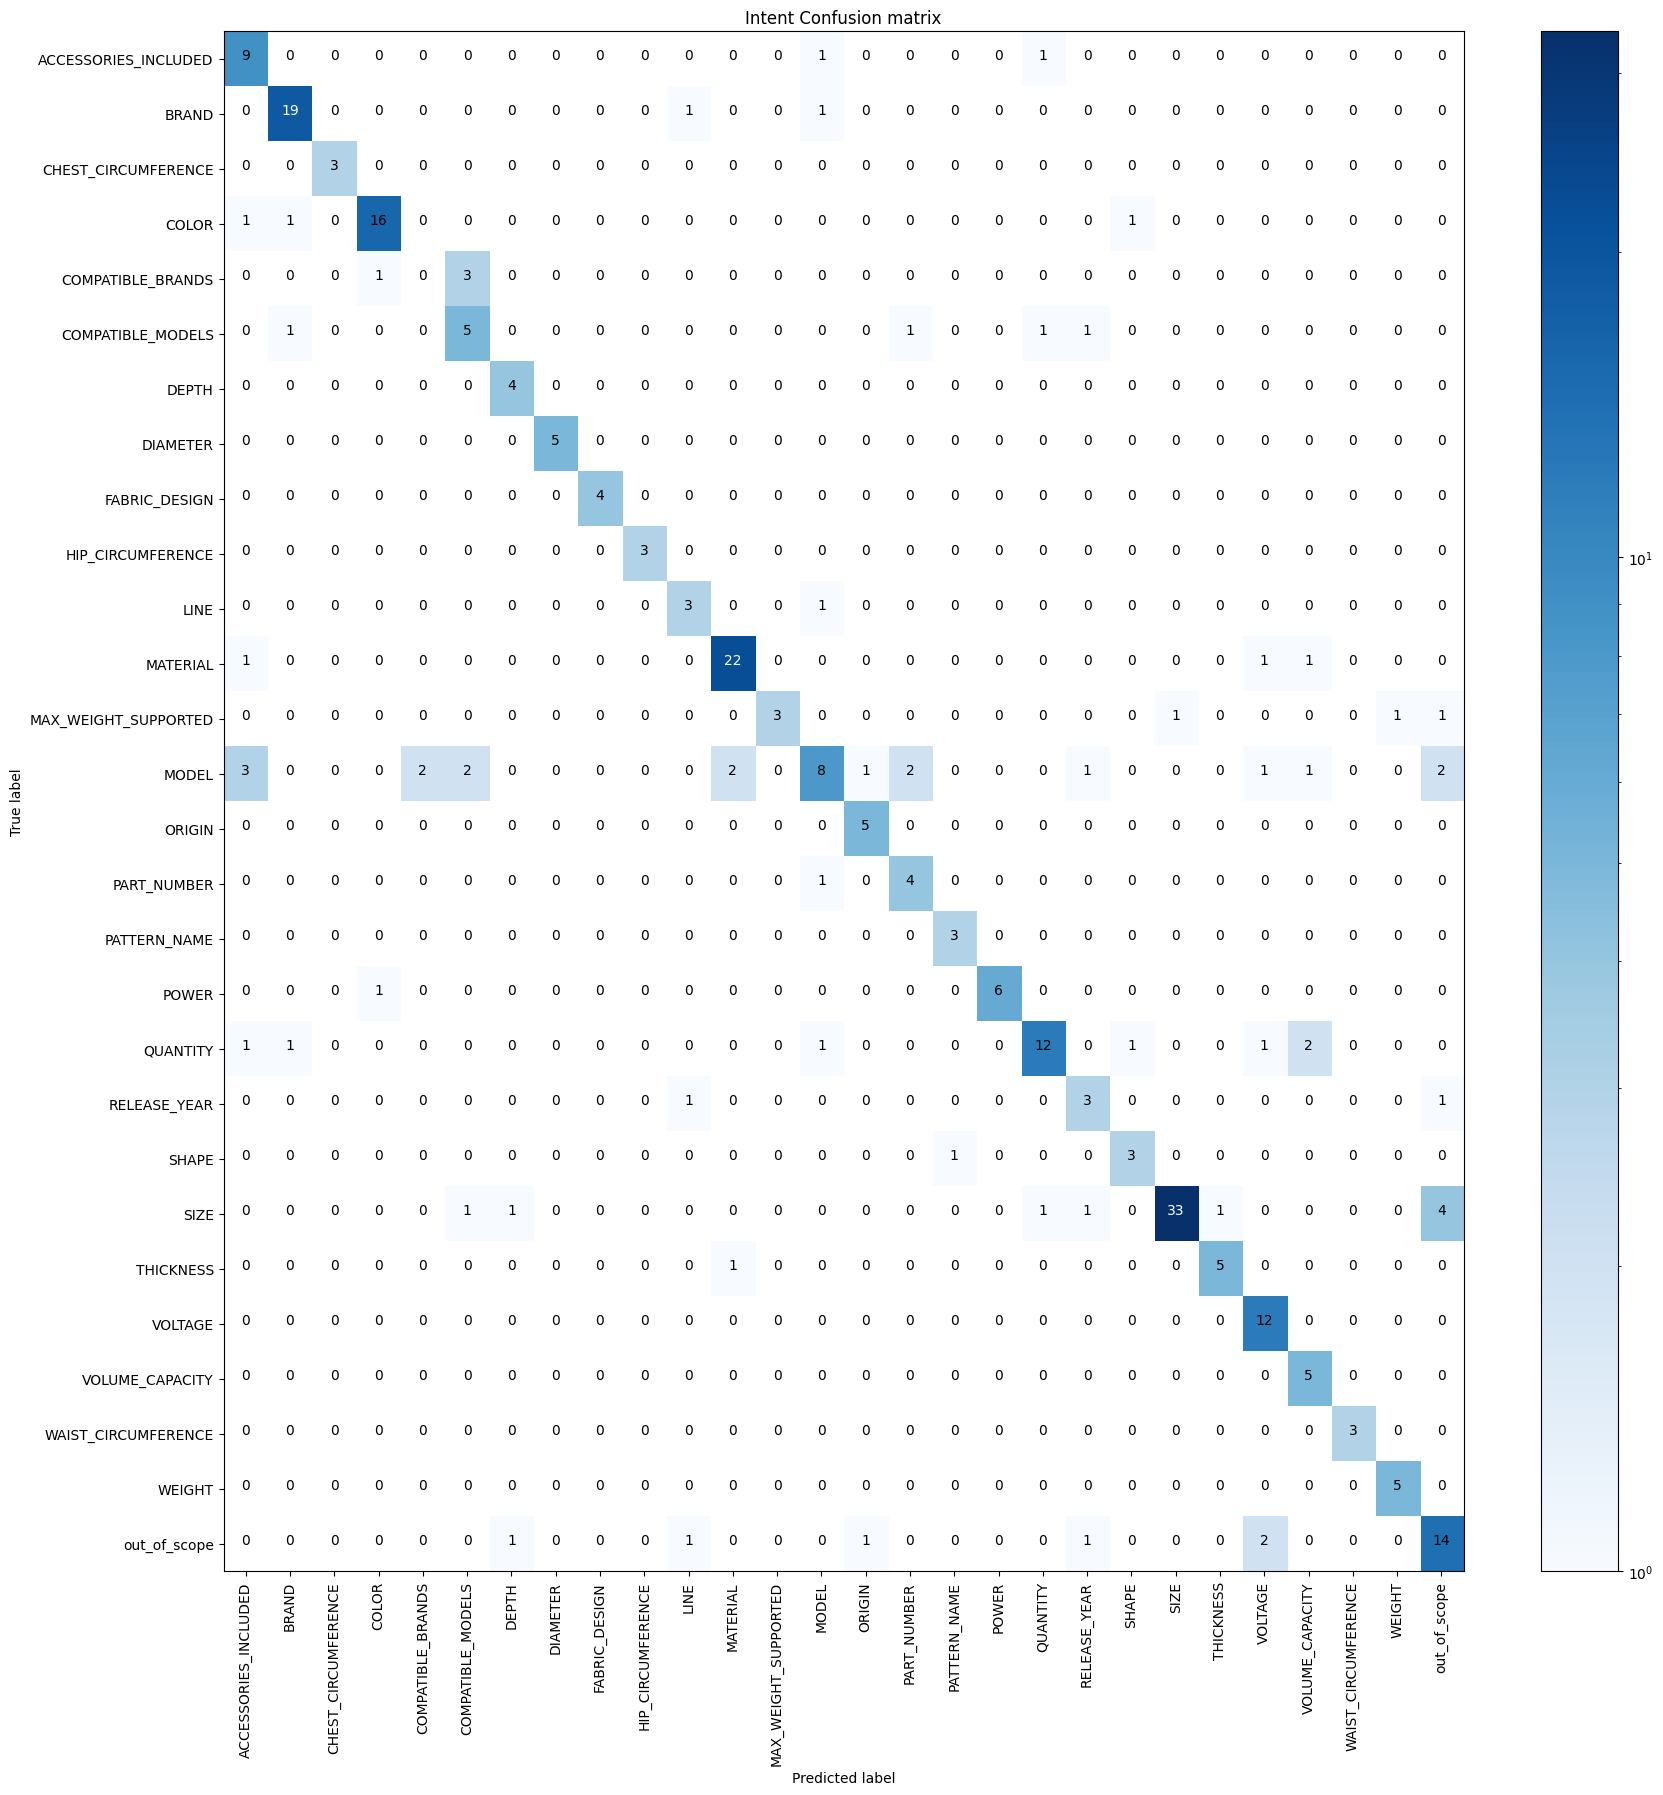
\includegraphics[width=1\linewidth]{figuras/RASA3-28_classes.png}
	\caption{Matriz de Confusão gerada após teste do modelo RASA3, na configuração com 28 classes.}
	\label{fig:matriz_rasa3_28_classes}
\end{figure}